\documentclass[aspectratio=169,t]{beamer}
\usepackage[czech]{babel}
\usepackage[utf8]{inputenc}
\usepackage[T1]{fontenc}
\usepackage{booktabs}
\usepackage{diagrams}
\usetheme[workplace=fi]{MU}
\title{Vektorové reprezentace ve vyhledávání znalostí}
\subtitle{Vector Space Representations in Information Retrieval}
\author[V.\ Novotný]{Vít Novotný \\ witiko@mail.muni.cz}
\institute[FI MU]{Faculty of Informatics, Masaryk University}
\date{\today}
\subject{Presentation Subject}
\keywords{the, presentation, keywords}
\date{6.\ února 2017}

% Macro definitions.
\let\abbr\relax
\let\term\emph
\begin{document}

\begin{frame}[plain]
\maketitle
\end{frame}

\begin{frame}{Obsah}
\tableofcontents
\end{frame}

\section{Úvod}
\begin{frame}[label=introduction]{Úvod}
\begin{itemize}
  \item<1-> V~rámci výzkumné skupiny Math Information Retrieval (\abbr{MIR})
    jsem se ve spolupráci s~firmou RaRe Technologies zúčastnil druhého ročníku
    projektu \alert<1>{\abbr{TA} \abbr{ČR} Omega}.
  \item<2-> Cíl byl vyvinout \alert<2-3>{segmentující vyhledávač}
    nestrukturovaných textových dokumentů\only<2-3>:\only<4->.
  \only<4->{%
  \item<4-> V rámci projektu jsem dostal možnost prezentovat náš výzkum na \abbr{ACL}~2017.
  \item<5-> V návaznosti na výzkum prezentovaný na \abbr{ACL}~2017 jsem
    provedl \alert<5->{dvojici experimentů}, které jsou předmětem této
    diplomové práce:
  \begin{enumerate}
    \item<6-> U~vyhledávačů, které musí vždy navrátit celé dokumenty a nikoliv
      pouze segmenty, lze \alert<6>{agregací nalezených segmentů} zlepšit
      kvalitu výsledků oproti hledání bez segmentace.
    \item<7-> Rozšířením standardního vektorového modelu o neortogonalitu mezi
      bázovými vektory lze \alert<7>{modelovat synonymitu slov} a docílit
      dalšího zlepšení kvality výsledků.
  \end{enumerate}}
\end{itemize}
\only<1-3>{%
  \only<3>{\hspace*{-14cm}}%
  \uncover<2-3>{\STqueryingdiagram}}
\only<4->{\vspace*{2cm}}
\end{frame}

\section{Datová sada}
\begin{frame}<1-4>[label=dataset]{Datová sada}
\begin{itemize}
\item<1-> V rámci obou experimentů jsem využil datovou sadu pro úlohu 3
  (zodpovídání dotazů) z~ročníků 2016 a 2017 soutěže SemEval.
\item<2-> Datové sady pro podúlohu 3a obsahují \alert<2-6>{vlákna s dotazem a
  prvními deseti komentáři} spolu s~anotací, jestli \alert<2-6>{je komentář
  relevantní k~dotazu}.
  \begin{itemize}
    \item<3-> Mike Godwin roku 1991 formuloval empirické pravidlo, že
      „s~rostoucí délkou UseNetové diskuze se pravděpodobnost přirovnání
      zmiňujícího nacisty nebo Hitlera blíží k~jedné.“
    \item<4-> Na základě tohoto pravidla jsem formuloval a vyvrátil hypotézu, že
      \alert<4>{pravděpodobnost výskytu relevantních komentářů na jednotlivých
      pozicích je rovnoměrná}.
  \end{itemize}
\item<5-> Datové sady pro podúlohu 3b obsahují dotazy a \alert<5-6>{pro každý
  dotaz deset vláken} spolu s anotací, jestli se \alert<5-6>{vlákno týká dotazu}.
  \begin{itemize}
    \item<6-> Tyto datové sady byly použity pro evaluaci v obou následujících
      experimentech.
  \end{itemize}
\end{itemize}
\end{frame}

\begin{frame}[c]
\begin{figure}
\vfill
\begin{center}
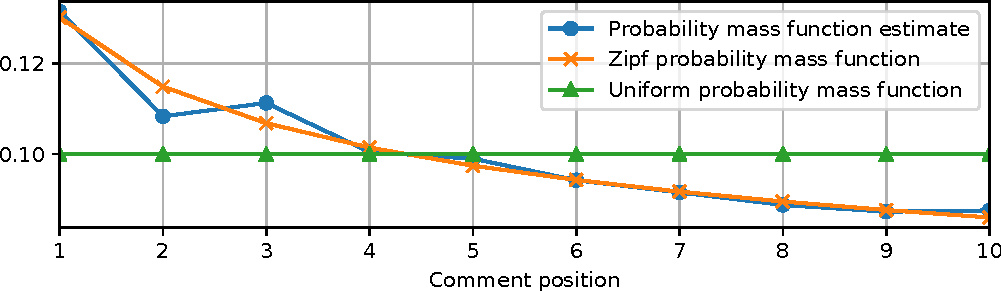
\includegraphics[scale=0.8]{figs/quality-evaluation-1.pdf}
\caption{Odhad pravděpodobnostní funkce $P(\text{na pozici }i\mid\text{relevantní})$
  vyobrazený modře spolu s~pravděpodobnostními funkcemi Zipfova (oranžový graf)
  a rovnoměrného rozdělení (zelený graf).}
\end{center}
\end{figure}
\end{frame}

\againframe<4->{dataset}

\section{Segmentované vyhledávání}
\begin{frame}<1>[label=segmentation]{Segmentované vyhledávání}
\begin{itemize}
  \item<1-> Vyhledávač navržený v projektu Omega indexuje a navrací
    \alert<1>{tématicky koherentní segmenty dokumentů}. Vyhledávače však často
    musí navracet celé dokumenty.
  \item<2-> V rámci experimentu jsem vyhledávač rozšířil o komponentu, která
    \alert<2>{agreguje podobnost segmentů vůči dotazu} do odhadu podobnosti
      dokumentu vůči dotazu.
    \begin{itemize}
      \item<3-> \alert<3>{Vlákna představují dokumenty}, \alert<3>{dotaz a
        komentáře uvnitř vláken představují segmenty}.
      \item<3-> S ohledem na analýzu datových sad podúlohy 3a je hlavním agregačním
        mechanismem \alert<3-4>{vážený průměr s~vahou $i^{-1}$ pro komentář na
        pozici $i$}. Tento mechanismus porazil nad datovými sadami pro ročníky
        2016 i 2017 vítěze soutěže.
      \item<4-> Pro srovnání byl otestován i \alert<4>{vyhledávač bez segmentace},
        který analogickým způsobem \alert<4>{váží jednotlivá slova dokumentu}.
        Tento vyhledávač byl poražen baseline výsledkem.
      \item<5-> Pro srovnání byl otestován i \alert<5>{vyhledávač bez segmentace},
        který \alert<5>{z~vlákna zachovává pouze úvodní dotaz}. Tento
        vyhledávač porazil baseline výsledek, ale ne vítěze soutěže.
    \end{itemize}
\end{itemize}
\end{frame}

\againframe<3>{introduction}
\againframe<1-4>{segmentation}

\begin{frame}[c]
\begin{figure}
\vfill
\begin{center}
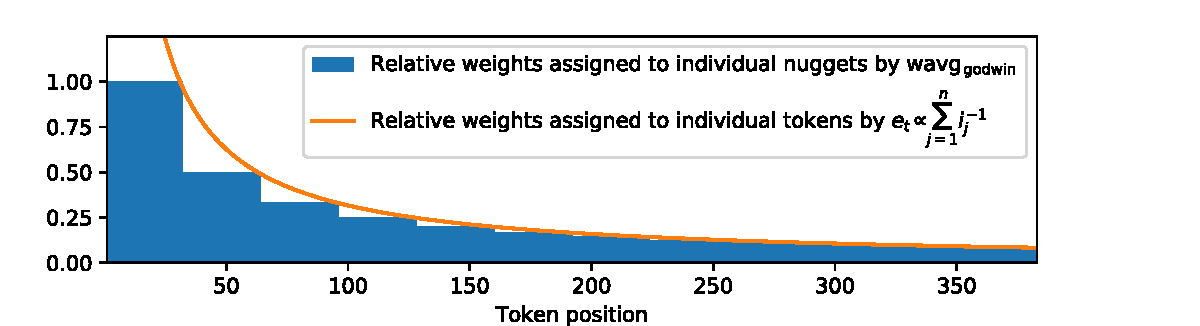
\includegraphics[trim={0.8cm 0.0cm 2.8cm 0.5cm}, scale=0.8]{figs/quality-evaluation-4.pdf}
\caption{Poměrný dopad jednotlivých slov v dokumentu na výsledný odhad
  podobnosti při váženém průměru jednotlivých segmentů (modře vyplněný graf) a
  při váženém průměru jednotlivých slov (oranžový graf).}
\end{center}
\end{figure}
\end{frame}

\againframe<4->{segmentation}

\section[Short Section 1 Name]{Full Section 1 Name}
\subsection[Short Subsection 1 Name]{Full Subsection 1 Name}

\begin{frame}{Frame Title}{Frame Subtitle}
plain text, \structure{page structure}, \alert{emphasis}
\begin{itemize}
  \item a single-line bullet list item
  \item a bullet list item that is quite long (in order to force a line break),
    which also contains \alert{emphasized text}
  \begin{itemize}
    \item a second-level list item
    \begin{itemize}
      \item a third-level list item
    \end{itemize}
    \alert{\item an emphasized second-level list item}
  \end{itemize}
\end{itemize}
\begin{enumerate}
  \item a numbered list item
  \begin{enumerate}
    \item a second-level list item containing a math expression
      \[ E = mc^2 \]
  \end{enumerate}
\end{enumerate}
\end{frame}

\subsection[Short Subsection 2 Name]{Full Subsection 2 Name}

\begin{frame}{Text Blocks}
text above a block
\begin{block}{Block}
  text
\end{block}
\begin{exampleblock}{Example Block}
  text
\end{exampleblock}
\begin{alertblock}{Emphasized Block}
  text
\end{alertblock}
text below a block\footnote{a footnote with an \url{http://address.edu}}
\end{frame}

\begin{frame}{Figures}
\begin{figure}
  \includegraphics[width=.5\textwidth,height=.5\textheight,keepaspectratio]{cow-black.mps}
  \caption{A Holstein Friesian cow}
\end{figure}
\end{frame}

\subsection[Short Subsection 3 Name]{Full Subsection 3 Name}

\begin{frame}{Tables}
\begin{table}
  \begin{tabular}{llc}
    First Name & Surname & Year of Birth \\ \midrule
    Albert & Einstein & 1879 \\
    Marie & Curie & 1867 \\
    Thomas & Edison & 1847 \\
  \end{tabular}
  \caption{The great minds of the 19th century}
\end{table}
\end{frame}

\makeatletter
\begin{frame}{Automatic Optical Scaling}
\begin{center}
\begin{tabular}{ll}
\Huge \f@family & \Huge \structure{\f@size pt} \\
\huge \f@family & \huge \structure{\f@size pt}  \\
\LARGE \f@family & \LARGE \structure{\f@size pt}  \\
\Large \f@family & \Large \structure{\f@size pt}  \\
\large \f@family & \large \structure{\f@size pt}  \\
\normalsize \f@family & \normalsize \structure{\f@size pt}  \\[-0.95pt]
\small \f@family & \small \structure{\f@size pt}  \\[-1.95pt]
\footnotesize \f@family & \footnotesize \structure{\f@size pt} \\[-2.95pt]
\scriptsize \f@family & \scriptsize \structure{\f@size pt}  \\[-4.95pt]
\tiny \f@family & \tiny \structure{\f@size pt}
\end{tabular}
\end{center}
\end{frame}
\makeatother

\begin{frame}[plain]
\vfill
\centerline{Děkuji vám za pozornost.}
\vfill
\end{frame}

\end{document}
